\chapter{TiveJS}
    In questo lavoro, come introdotto, presento TiveJS, che è un porting ed un'evoluzione di Tive e come esso è in grado di: permettere la progettazione di sentenze visive grazie all'ausilio di palette di simboli personalizzate, il riconoscimento di linguaggio diagrammatici e la traduzione di quest'ultimi.
    \newline
    Il paper da cui deriva questo lavoro è \textit{Using the local context for the definition and implementation of visual languages}~\cite{localcontext} in cui si parla di un metodo per la traduzione di diagrammi o in generale di sentenze visuali in sentenze semantiche.
    \section{Funzionamento e Implementazione}
        Il funzionamento si suddivide principalmente in tre fasi, mostrate schematicamente nella figura~\ref{fig:funzionamento}: la progettazione del diagramma, il riconoscimento di quest'ultimo e l'applicazioni delle definizioni sintattiche e semantiche.
        \newline
        \begin{figure}
            \centering
            \smartdiagramset{border color=none,
                back arrow disabled=true,
                text width=3.5cm,
                module minimum width=3.5cm,
                module x sep=5
            }
            \smartdiagram[flow diagram:horizontal]{Progettazione, Riconoscimento, Applicazione Definizioni}
            \caption{Diagramma del funzionamento di TiveJS}
            \label{fig:funzionamento}
        \end{figure}
        Come vedremo, ogni fase può suddividersi in più sotto-fasi illustrate nel dettaglio nelle prossime sezioni.
        
        \subsection{Progettazione di sentenze visive}
            La progettazione delle sentenze visive avviene attraverso una GUI\footnote{Interfaccia Grafica.} molto semplice ed intuitiva, simile a quella nella figura~\ref{fig:drawio}.

            \begin{figure}[htbp]
                \centering
                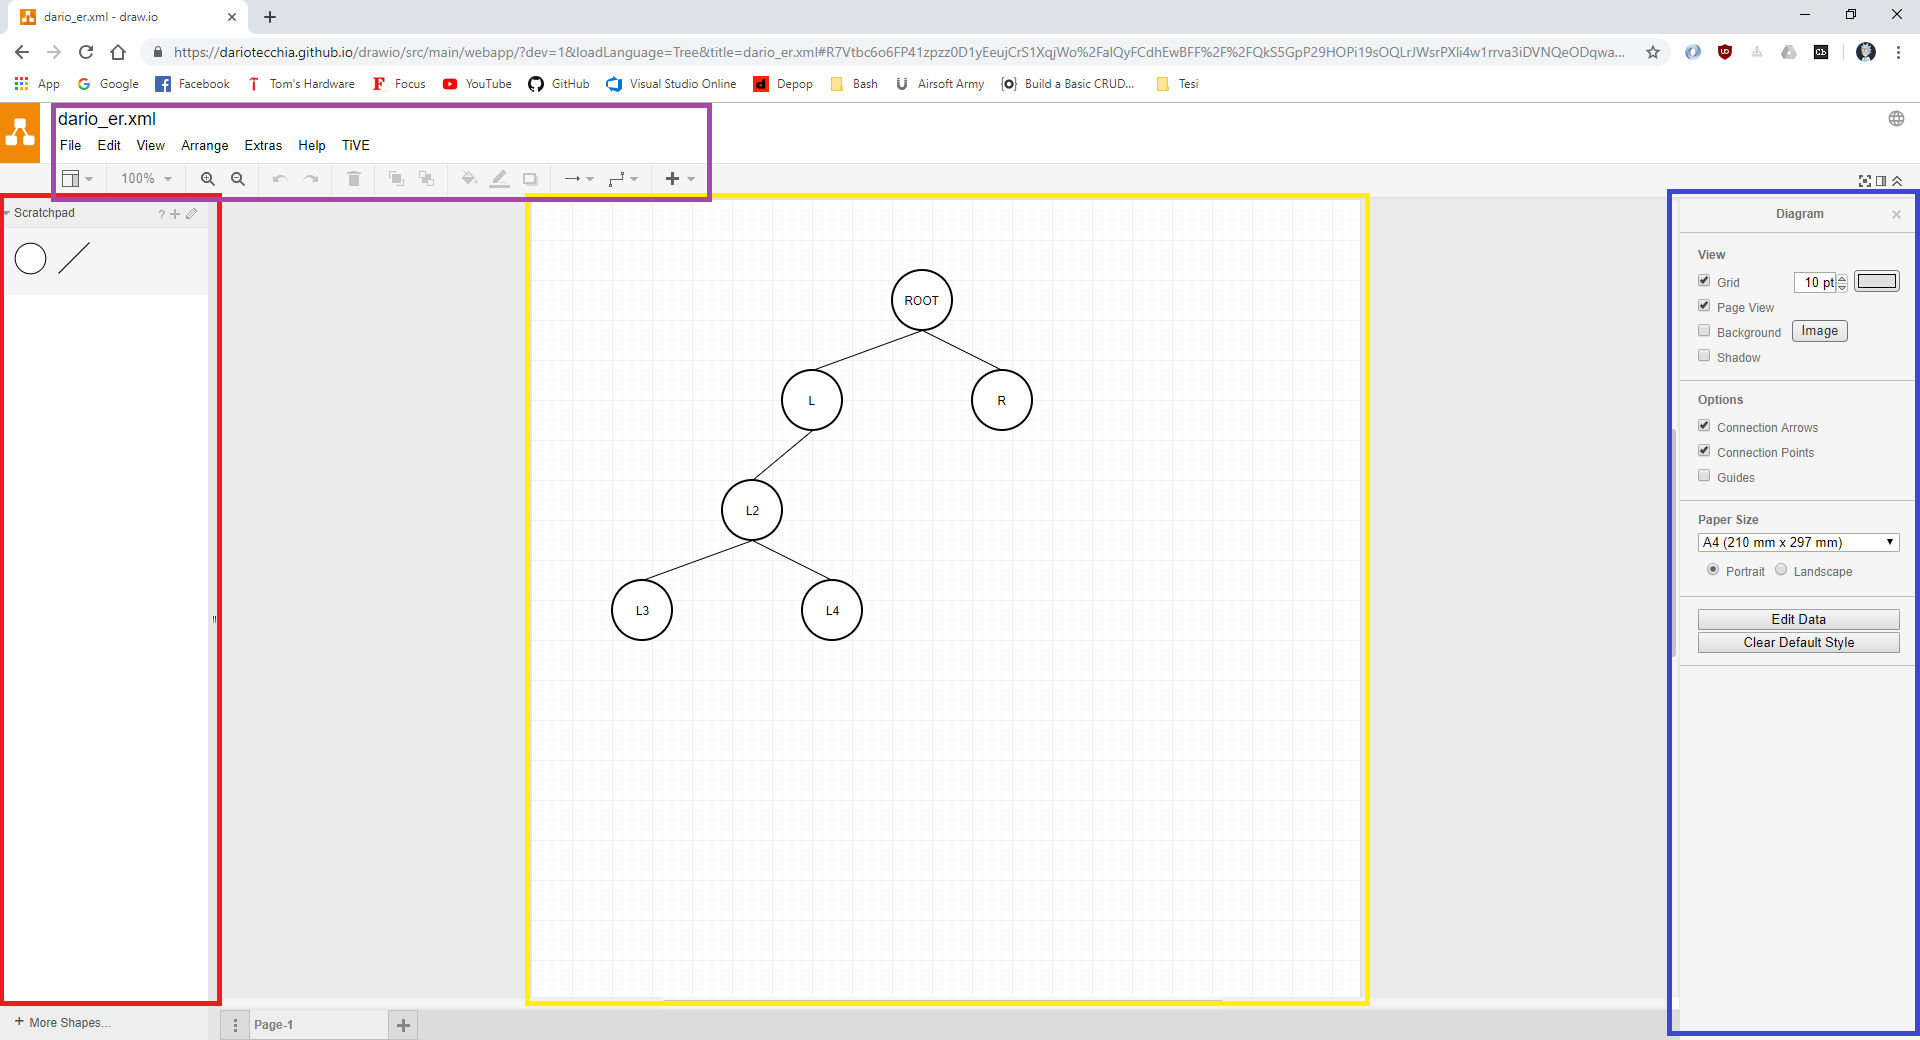
\includegraphics[scale=0.25]{Figure/tivejs_gui2.png}
                \caption{Schermata principale di TiveJS}
                \label{fig:tivejsgui}
            \end{figure}

            E' composta di quattro sezioni principali (figura~\ref{fig:tivejsgui}):
            \begin{itemize}
                \item Barra laterale sinistra (evidenziata \textcolor{red}{rosso})
                \item Barra laterale destra (evidenziata \textcolor{blue}{blu})
                \item Area di lavoro (evidenziata \textcolor{yellow}{giallo})
                \item Barra dei menu (evidenziata \textcolor{purple}{viola})
            \end{itemize}
            All'interno della barra laterale sinistra troviamo la palette dei simboli importata precedentemente creata con l'ausilio di \textit{drawSE}. Per importare una nuova librearia (o palette) bisogna andare nel menu \textit{File -> Open Library From} e selezionare il metodo di importazione.
            \newline
            La barra laterale destra serve personalizzare ulteriormente il diagramma o il singolo simbolo. Mette a disposizione vari menù ed opzioni quali la dimensione della pagina su cui disegnamo il diagramma, colore di un simbolo, le proprietà del testo contenuto all'interno di un simbolo, ecc. 
            \newline
            L'area di lavoro è dove viene composto il diagramma trascinando i simboli dalla barra laterale. All'interno di quest'area possiamo selezionare, modificare e spostare il diagramma e i relativi simboli a nostro piacimento.
            \newline
            La barra dei menu è composta da tanti sotto menu ognuno dei quali ha una funzione specifica. Oltre ai menu di draw.io è stato aggiunto un nuovo menu "TiVE" (figura \ref{fig:tivemenu}) per il caricamento delle definizioni e per la verifica del grafo. Nello specifico, "\textit{Load Rules...}" serve per il caricamento delle definizioni sintattiche; "\textit{Load Semantic Rules...}" per il caricamento delle definizioni semantiche e "\textit{Apply Rules}" eseguire l'applicazione di quest'ultime e la traduzione del diagramma.
            
            \begin{figure}[htbp]
                \centering
                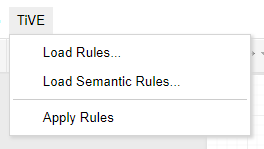
\includegraphics[]{Figure/tive_menu.PNG}
                \caption{Menu dei comandi per TiVE}
                \label{fig:tivemenu}
            \end{figure}

        \subsection{Riconoscimento grafo}
            All'interno di diagramma più simboli con scopi diversi possono condividere lo stesso elemento grafico creando delle ambiguità. Una delle prime fasi del processo di traduzione è il riconoscimento degli elementi e quindi la risoluzione di queste ambiguità. Come possiamo notare nella tabella~\ref{tab:final_syntax_definition}, in particolare nella seconda sotto-tabella, i connettori pur avendo uno scopo diverso condividono lo stesso elemento grafico, una linea.
            \newline
            Ancora, nella tabella \ref{tab:final_syntax_definition_tree} a condividere lo stesso elemento grafico è un simbolo: radice e nodo sono entrambi rappresentati da un cerchio.

            \begin{table}[htbp]
                \centering
                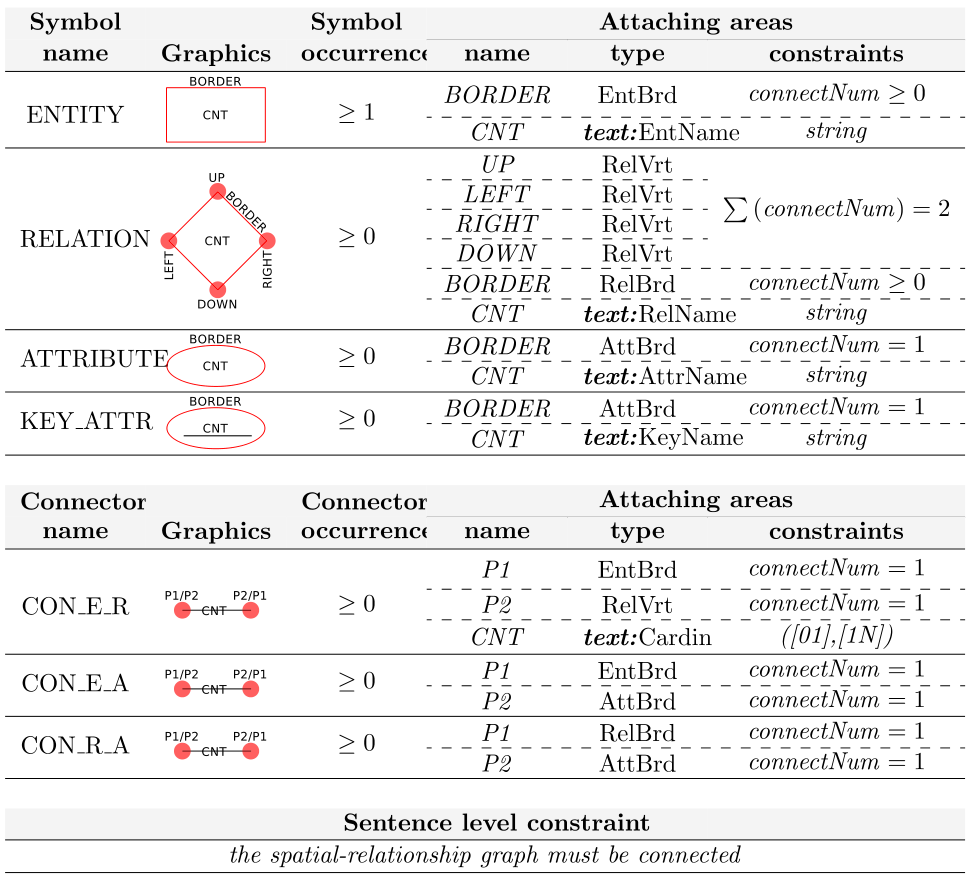
\includegraphics[scale=0.4]{Figure/final_syntax_definition.PNG}
                \caption{Specifica di un diagramma ER}
                \label{tab:final_syntax_definition}
            \end{table}

            \begin{table}[htbp]
                \centering
                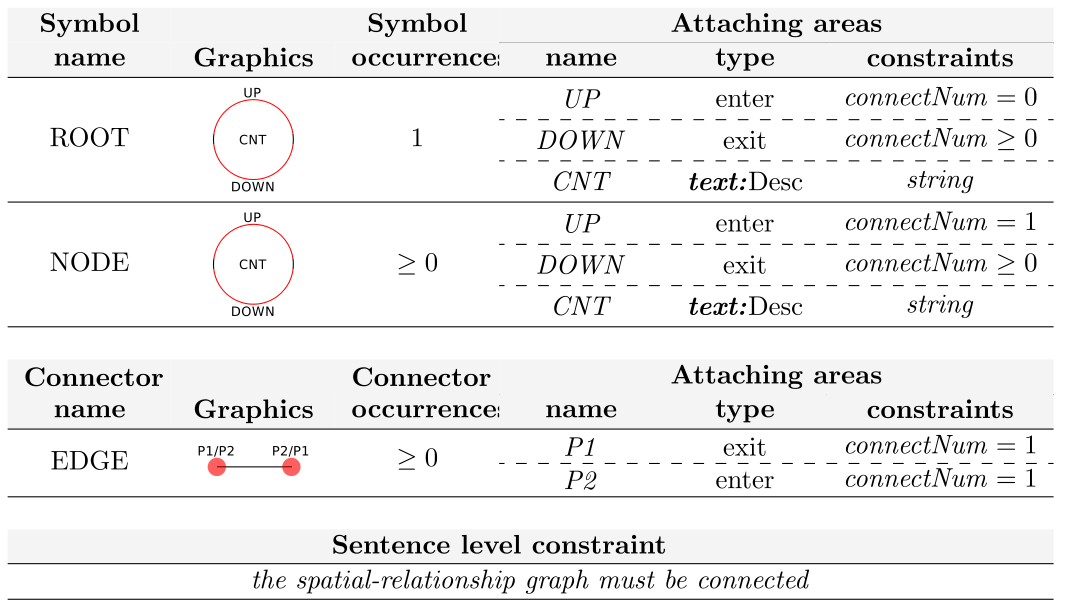
\includegraphics[scale=0.4]{Figure/final_syntax_definition_tree.PNG}
                \caption{Specifica di un Albero}
                \label{tab:final_syntax_definition_tree}
            \end{table}

            A caratterizzare un elemento sono le proprietà della definizione sintattica correlata. La disambiguazione viene effettuata tenendo in considerazione questi elementi.
            \newline
            L'algoritmo risolutivo innanzitutto rileva se si sta analizzando un vertice o un connettore e nel caso in cui venissero rivelate delle ambiguità procede come segue: Se l'elemento analizzato è un connettore prende in considerazione il campo \textit{Type} delle due aree d'attacco. All'interno di questa proprietà vengono indicati i tipi di area d'attacco in cui il connettore è collegato alle due estremità. Ad esempio, il connettore \textit{CON\_E\_A} (Connettore Entità-Attributo) alle due estremità si connetterà ad una \textit{EntBrd} e ad una \textit{AttBrd} in posizioni arbitrali; Nel caso un cui l'elemento analizzato è un vertice allora il controllo viene effettuato sui vincoli definiti per ogni simbolo. Il vertice sarà associato al simbolo per cui verranno rispettate tutti i suoi vincoli. Ad esempio, il simbolo \textit{Root} dovrà avere un numero di connessioni (\textit{connectNum}) uguali a zero sull'attaching area UP di tipo enter e un numero maggiore o uguale a zero di connessioni sull'attaching area DOWN di tipo exit.
            \newline

        \subsection{Applicazione definizioni}
            Eseguito il riconoscimento ogni simbolo appartenente al grafo si può procedere con l'applicazione delle definizioni. Come ho già accennato, la specifica delle definizioni si divide in due parti: sintattica e semantica.

            \subsubsection{Definizioni Sintattiche}
                Ogni linguaggio ha delle regole sintattiche da rispettare. Un esempio di definizione sintattica è raffigurata nella tabella \ref{tab:final_syntax_definition}, nella colonna \textit{Symbol occurences} vi è un vincolo al livello del simbolo, indica quante occorrenze del simbolo devono essere presenti all'interno del diagramma. Nell'ultima colonna, \textit{constraints}, vi troviamo i vincoli al livello degli Attaching Point e il formato che deve avere il campo di testo dell'elemento se specificato. Nell'ultima riga, \textit{Sentence level constraint}, troviamo i vincoli che il diagramma deve rispettare.
                \newline
                Come ho già accennato, in Tive le definizioni erano scritte in formato XML (vedi Appendice \ref{appendix:xml_definition}). Successivamente sono state implementate in formato JSON\footnote{JavaScript Object Notation} per poter essere interpretate in maniera nativa dal linguaggio di programmazione usato. All'interno dello snippet di codice \ref{lst:newDefinition} vi è una parte della definizione nel nuovo formato. 
                \newline
                Il valore di "\textit{ap}" è un array contenente i vincoli per i punti d'attacco; "\textit{text}" contiene le informazioni riguardanti le aree di testo, "\textit{\_name}" è il nome del simbolo; "\textit{\_ref}" indica a quale figura grafica si fa riferimento; "\textit{occurences}" è il vincolo sulle occorrenze del simbolo.
                \newline
                L'intera definizione è consultabile all'Appendice \ref{appendix:jsonDefinition}.
                \newpage
                \begin{spacing}{0.5}
                    \lstinputlisting[caption={\textbf{Frammento della definizione in formato JSON di un linguaggio, nel particolare la specifica per il simbolo \textit{ROOT} (o Radice).}},label={lst:newDefinition}, firstline=4, lastline=29]{SourceCode/newDefinition.json}
                \end{spacing}

            \subsubsection{Definizioni Semantiche}
            
                
        \subsection{Traduzione}

    \section{Tecnologie Utilizzate: JavaScript}
        TiveJS è stata implementata completamente in JavaScript per far si che potesse girare su ogni browser web.
        JavaScript, a volte abbreviato con JS, è un linguaggio di programmazione interpretato ad alto livello. Standardizzato per la prima volta nel 1997 con il nome di ECMAScript (attualmente l'ultima release è ECMAScript 2018~\cite{ecmascript}), insieme all'HTML e il CSS è una delle tecnologie alla base del World Wide Web.
        In questa sezione esaminiamo alcuni dei punti di forza di JavaScript, così da capire quali sono le sue particolarità.

        \subsection{Punti di Forza di JavaScript}

            \subsubsection{Ricco di librerie}
                JavaScript, oltre le sue librerie standard, conta un numero impressionante di librerie scritte da una community molto attiva. Dispone di API per lavorare con testo, matrici, date, espressioni regolari e DOM\footnote{Document Object Model}.

            \subsubsection{Supporto universale}
                Tutti i moderni browser web supportano nativamente JavaScript con gli interpreti implementati al loro interno.
            
            \subsubsection{Multi-paradigma}
                JavaScript è un linguaggio multi-paradigma, che supporta la programmazione basata sugli eventi, la programmazione funzionale e quella imperativa (inclusa la programmazione orientata agli ogetti).

            \subsubsection{Portabile}
                JavaScript è un linguaggio portabile. E' possibile usarlo su diverse piattaforme come: \textit{Linux, Windows, OSx, iOS e Android}. Questo è possibile perchè non dipende dalla macchina dove gira essendo interpretato e non compilato. E' necessario però un interprete JavaScript.

            \subsubsection{Semplice}
                Molto semplice da imparare e perfetto da usare come linguaggio accademico essendo ad un linguaggio ad alto livello.

            \subsubsection{Gratis}
                JavaScript è totalmente gratis ed è possibile utilizzarlo e distribuirlo senza restrizioni di copyright. Nonostante questo, alle spalle ha una community attivissima.

        \subsection{Principali Applicazioni}
            Pur essendo un linguaggio rilasciato per i browser web, Netscape, nel 1995 introdusse una nuova implementazione del linguaggio per lo scripting server-side. Una delle implementazioni server-side più famosa è Node.js.

        \section{Librerie utilizzate nel Progetto}
            \subsubsection{mxGraph}
                Come accennato, una delle librerie utilizzate all'interno di TiveJS è mxGraph. Serve per lo sviluppo di diagrammi e permette la creazione di applicazioni interattive per la creazione di grafi e diagrammi. Oltre che in JavaScript è scritta anche in linguaggi server side quali PHP, .NET e Java~\cite{mxgraph}.
            \subsubsection{jQuery}
                jQuery risulta essere la libreria JavaScript più utilizzata su Internet per via della facilità di installazione e utilizzo.
                \newline
                Lo slogan di jQuery non a caso è \textit{<<write less, do more>>} poichè nasce con l'intenzione di semplificare la selezione, la manipolazione, la gestione degli eventi e l'animazione di elementi DOM in pagine HTML, nonchè implementare funzionalità AJAX~\cite{jquery}.
                \newline
                Da agli sviluppatori un'interfaccia semplice, accessibile attraverso il caratteristico simbolo \textbf{\$}, astraendo comandi molto più complessi offerti da JavaScript. E' un software libero.